
\chapter{Tubo di risonanza}

\section{Introduzione}

\section{Strumentazione}
\subsubsection{Tubo aperto contente aria}
Dati geometrici tubo:\\
$L = 90\pm 0.5\ cm$\\
$d = 3.9\pm 0.1\ cm$\\
con $L$ lunghezza e $d$ diametro del tubo.

\section{Tubo aperto contenente aria}
Cerchiamo le frequenze cui corrisponde, sullo schermo dell'oscilloscopio, il segnale massimo: in tal caso si ha la condizione di risonanza. Vogliamo verificare che tali valori stiano fra loro come multipli interi, secondo la legge:

\begin{equation} \label{eq:gianni}
\nu_n= n\frac{v}{2L} \hspace{3cm} n\in\mathbb{N} = \lbrace 1,2,3 \dots \rbrace
\end{equation}
con $v$ velocità del suono nel mezzo.
\\
Di seguito i dati raccolti:
\begin{center}
\begin{tabular}{c|c|c|c|c|c}
$\nu$ (Hz) & 185 & 370 & 558 & 930 & 1320 \\
\midrule
$n$ & 1 & 2 & 3 & 5 & 7\\
\end{tabular}
\end{center}
Interpoliamo i dati con una retta, usando il metodo dei minimi quadrati. Poniamo $x_i=n_i$, $y_i=\nu_i$ ed $m=\displaystyle{\frac{v}{2L}}$. Per stabilire l'errore sulle $y$, ossia sulle frequenze, si opera ad una analisi sperimentale della sensibilità dell'oscilloscopio; si verifica che all'interno di un intervallo minore di 10 Hz lo strumento non è in grado di distinguere ulteriori variazioni nella lettura delle frequenze: se ne ricava che l'incertezza relativa alle misure è di $\pm5 Hz$.

\begin{center}
<<<<<<< HEAD
%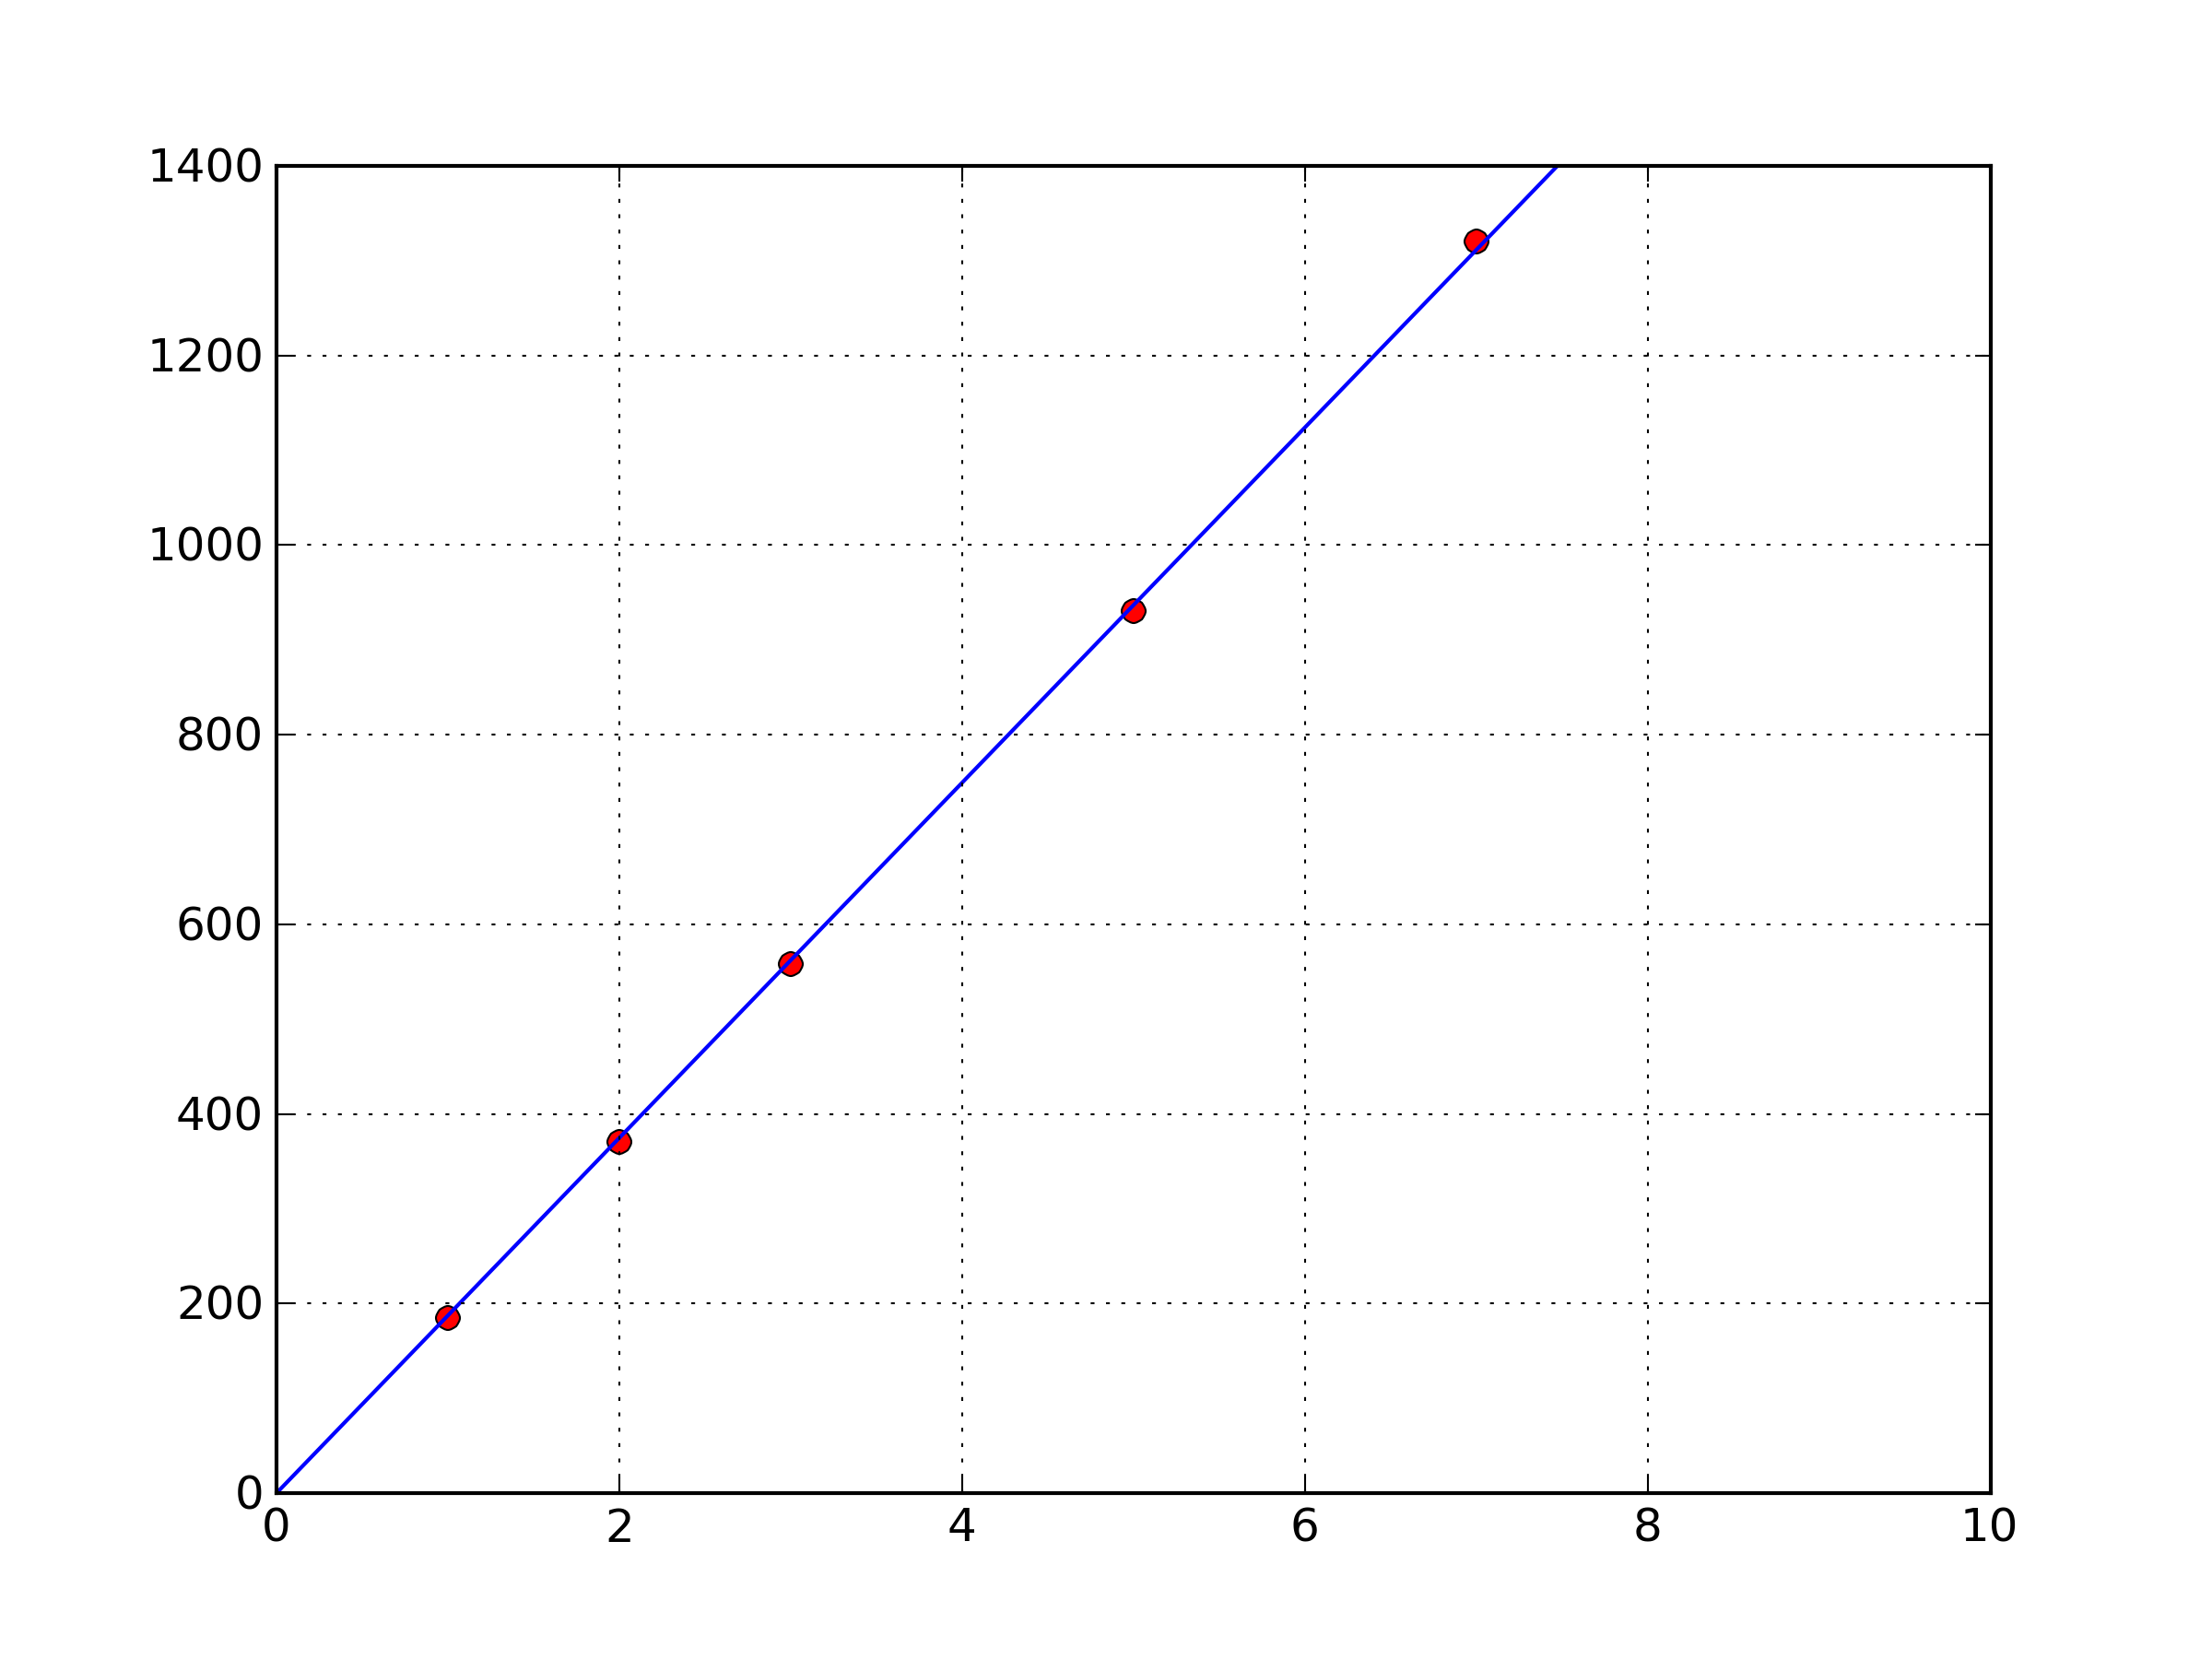
\includegraphics[scale=0.5]{../grafici/tubo/tubo1.pdf}

=======
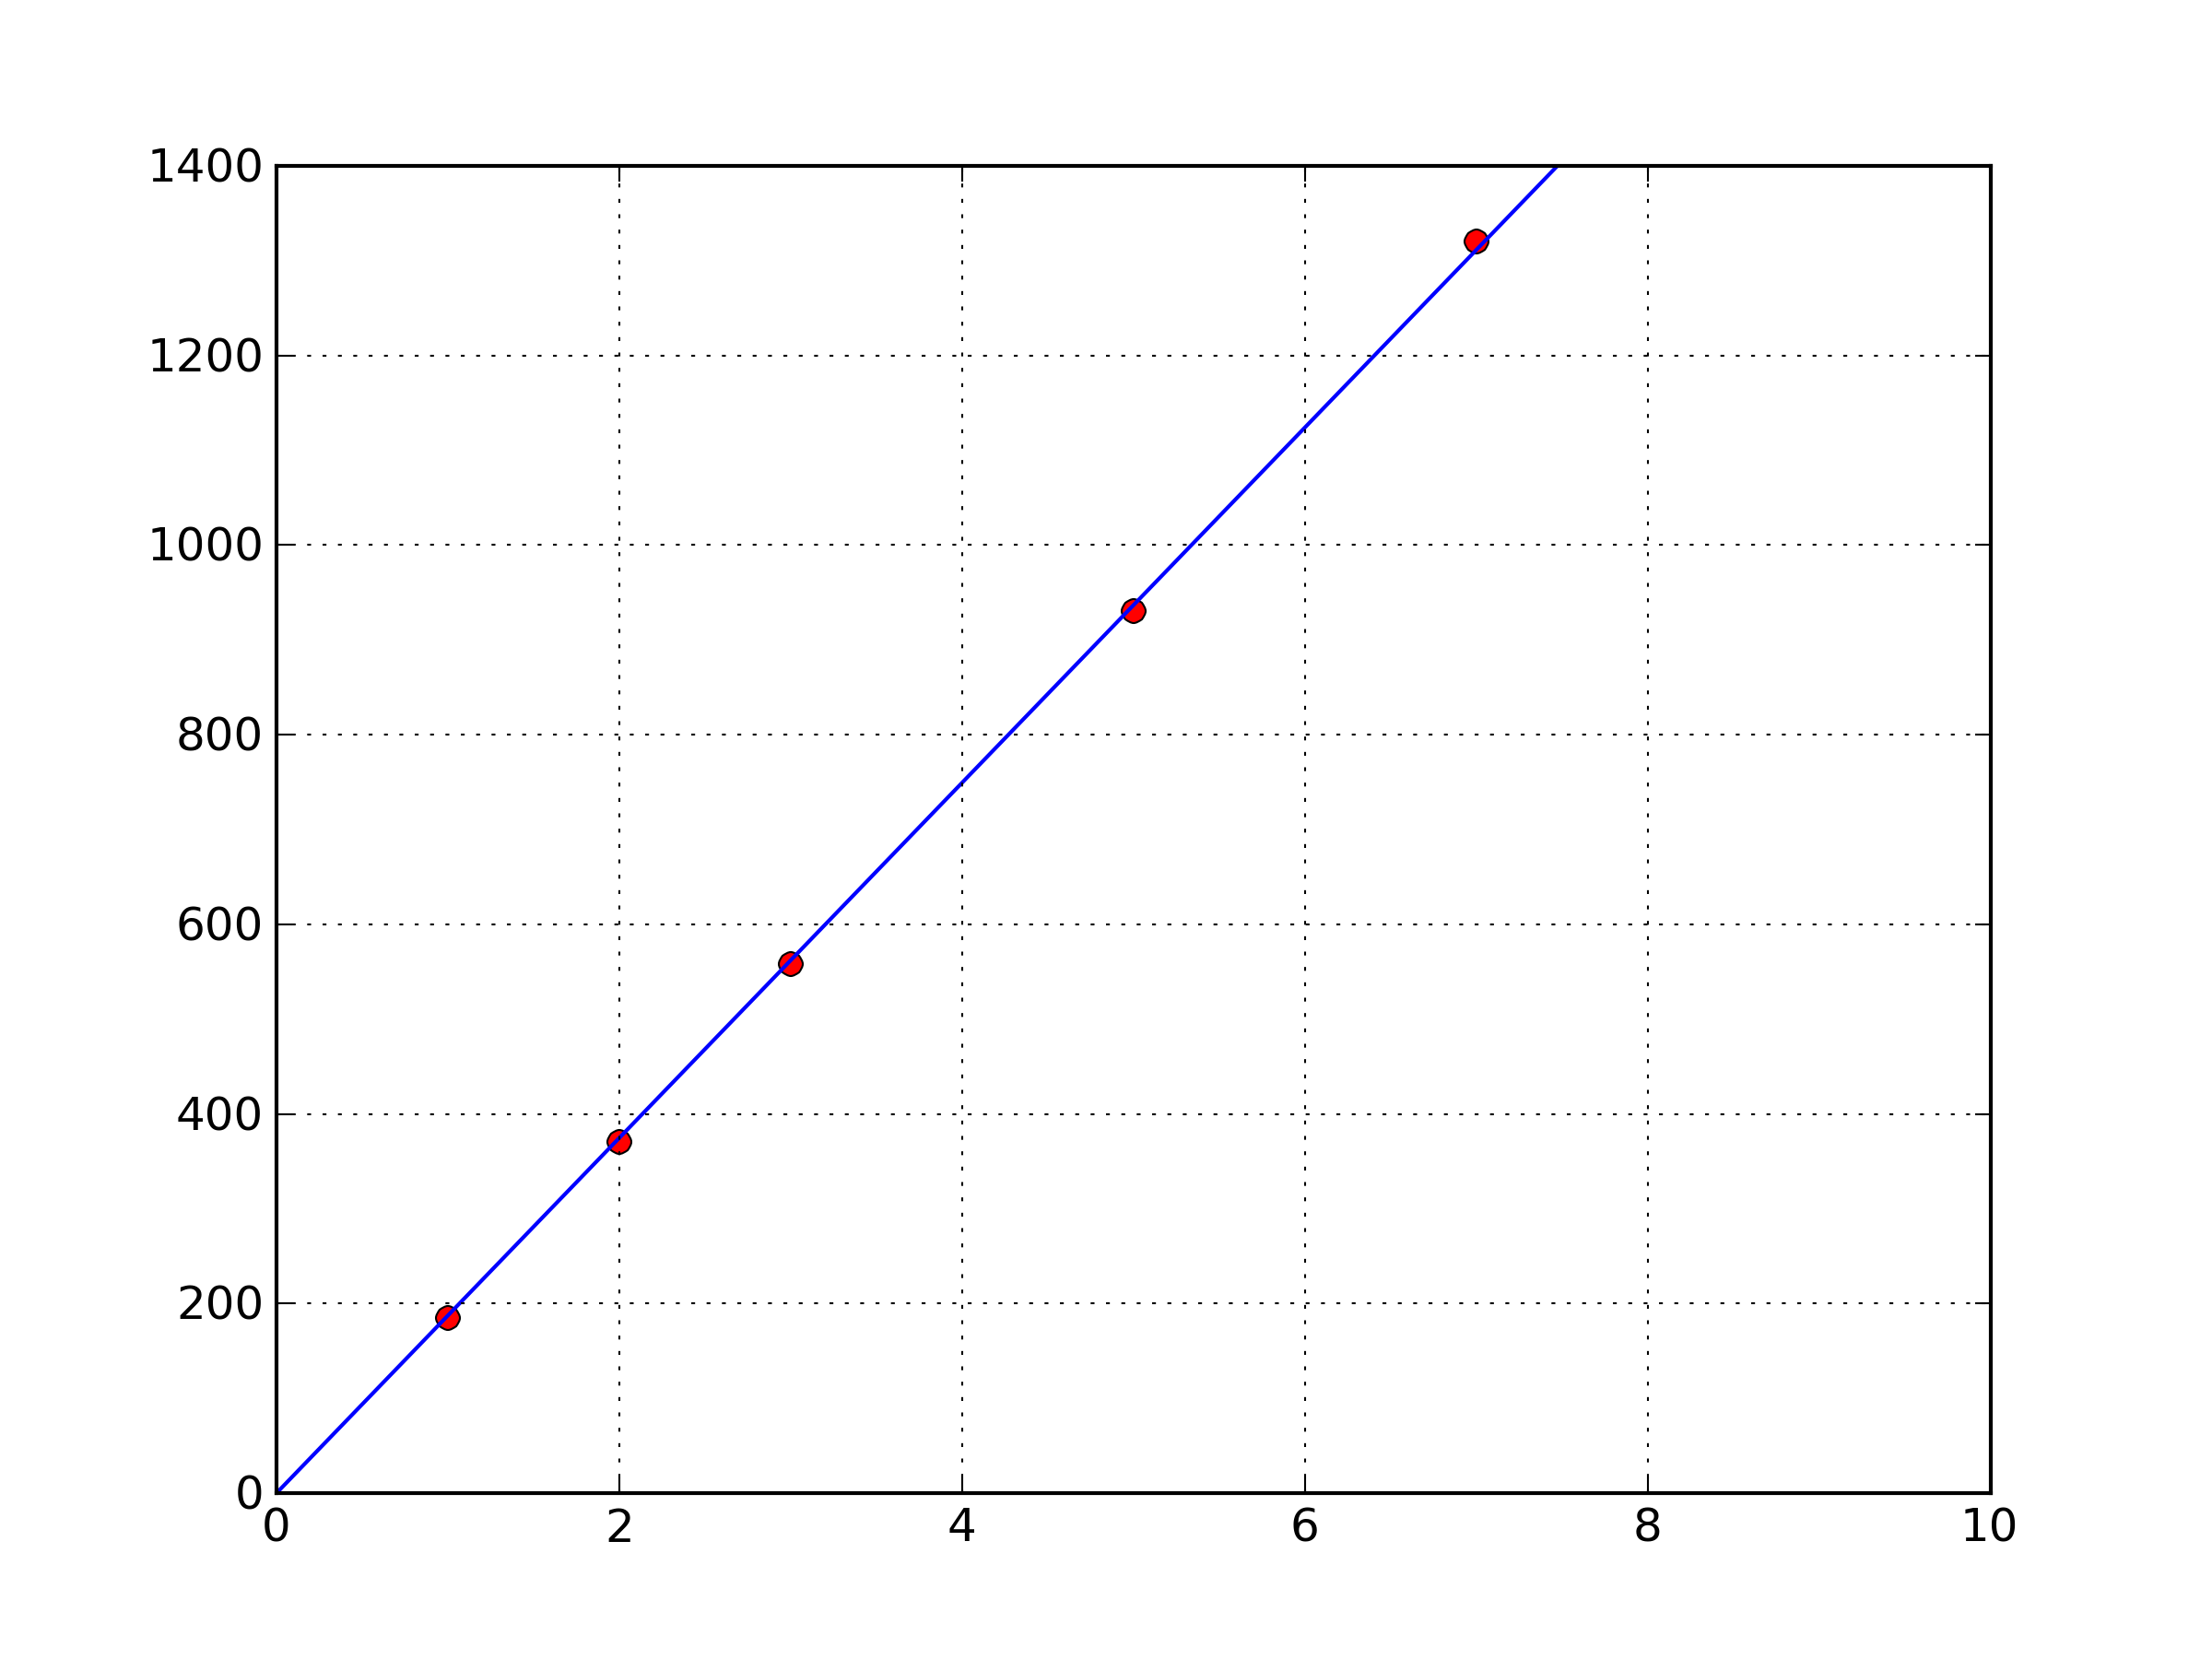
\includegraphics[scale=0.5]{../grafici/tubo/tubo1.png}
>>>>>>> 28c9e3f9b3f94c7ff3a9d06cf79cff91aed87615
$m = 187\pm 1\ s^{-1}$\hspace{1cm}\footnote{L'incertezza su $m$ è data da: $$\sigma_m=\frac{\sigma_y}{\sqrt{\sum{x_i^2}}}$$}
\end{center}

Verifichiamo l'accordo tra la funzione ed i dati sperimentiali con un test del $\chi^2$, ponendo la soglia di accettabilità al 5\%.
\begin{equation}\label{chi2}
\chi^2=\displaystyle{\frac{\sum{(y_i-mx_i)^2}}{\sigma_{y}^2}}
\end{equation}

ponedo $\sigma_{y_i}=5\ Hz$ e $d=4$ otteniamo: $\tilde{\chi}^2=1,75$. Allora la probabilità che $\chi^2\geq\tilde{\chi}^2$ è del 13\%, il che conferma la correttezza delle ipotesi fatte.\\
\\
Tuttavia per un tubo aperto reale, la posizione di nodi e antinodi dipende anche dal diametro del tubo, secondo la legge:
$$\frac{n\lambda}{2}=L+0.8d$$ pertanto, prima di calcolare $v$ dal valore di $m$ apportiamo la seguente correzione:
$$ L_c = (90\ cm)+(0.8)(3.9\ cm) = 93.12\ cm = 0.93 m $$
Si ricava dunque che $$v=2L_cm=348\pm0.02\ m/s$$
\\
L'errore è stato ricavato dalla propagazione degli errori sulle lunghezze e sull'interpolazione:
$$\sigma_{L+0.8D}=\sqrt{((\sigma_L)^2+(0.8\sigma_D)^2}=0.55\ cm$$
$$\sigma_v= \sigma_{2mL_c}= 2\sqrt{\left(\frac{\sigma_m}{m}\right)^2+\left(\frac{\sigma_{L_{c}}}{L_c}\right)^2}= 0.02\ m/s$$


%Si può ricavare $v$ direttamente dalla \ref{eq:gianni} (con la correzione), sostituendo a $\nu$ la frequenza fondamentale $\nu_0 = 185$ Hz

%$$ v = 2L_c\frac{\nu}{n} = 344.544\pm9.39\ m/s$$ 
Confrontiamo il valore ottenuto con quello previsto dalla legge:
\begin{equation}
v=\sqrt{\frac{\gamma R T}{M}} = 348\ m/s
\end{equation}
con $\gamma=\displaystyle{\frac{C_p}{C_v}}=\frac{7}{5}$ (gas biatomico), $R=8.31\ J/K mol$, $T=293\ K$, $M= 0.028\ kg/mol$ (massa molare dell'azoto $N$).


\subsection{Ventri e nodi}
Posta una frequenza corrispondente a $n>1$ ($n=2, n=3$), spostiamo all'interno del tubo il microfono e cerchiamo i punti corrispondenti a ventri e nodi (posizione rispetto all'inizio del tubo).

\begin{center}
\begin{tabular}{r r r r}

\multicolumn{2}{c}{$\nu$ = 370 Hz}& \multicolumn{2}{c}{$\nu$ = 558 Hz}\\
\textit{nodo 1}:& 0 cm & \hspace{2cm}\textit{nodo 1}:& 0 cm\\
\textit{ventre 1}:& 22.5 cm & \hspace{2cm}\textit{ventre 2}:& 15 cm\\
\textit{nodo 2}:& 45 cm &\hspace{2cm}\textit{nodo 2}:& 30 cm\\
\textit{ventre 2}:& 67.5 cm &\hspace{2cm}\textit{ventre 3}:& 45 cm\\
\textit{nodo 3}:& 90 cm &\hspace{2cm} \textit{nodo 3}:& 60 cm\\
& & \textit{ventre 4}:& 75 cm \\
& & \textit{nodo 4}:& 90 cm \\
\end{tabular}
\end{center}

Si verifica che essi corrispondono a quanto previsto dalla \ref{frequenza}: per $n=2$ si hanno tre nodi (uno all'inizio, uno alla fine ed uno al centro della corda) e due ventri (nei punti medi dei segmenti congiungenti due nodi consecutivi); analogalmente avviene per $n=3$, in cui si hanno 5 nodi e 3 ventri. \footnote{Abbiamo omesso in tabella di riportare tutte le incertezze, per renderla più leggibile. La precisione del metro a nastro è di $\pm1\ mm$.}

\section{Tubo chiuso ad una estremità, contenente aria}

La condizione per l'instaurarsi di onde stazionarie in un tubo chiuso ad una estremità è data dalla relazione:
\\
\begin{equation}
 L=(2n-1)\frac{\lambda}{4}
\end{equation}
\begin{equation}\label{freq2}
\nu=\frac{(2n-1)}{L}v
\end{equation}
Operativamente, abbiamo risolto l'equazione soprastante rispetto a $n$.

$$ n = \frac{2L_c\nu}{v} + \frac{1}{2} $$
Verifichiamo, come nel caso del tubo aperto, che le frequenze di risonanza stanno fra loro come multipli interi: 

\textbf{L = 90 cm}
\\
\begin{center}
\begin{tabular}{c|c|c|c|c|c}
$\nu$ (Hz) & 285 & 475 & 670 & 860 & 1050 \\
\midrule
$n$ & 2 & 3 & 4 & 5 & 6 \\
\end{tabular}
\end{center}


\begin{center}
%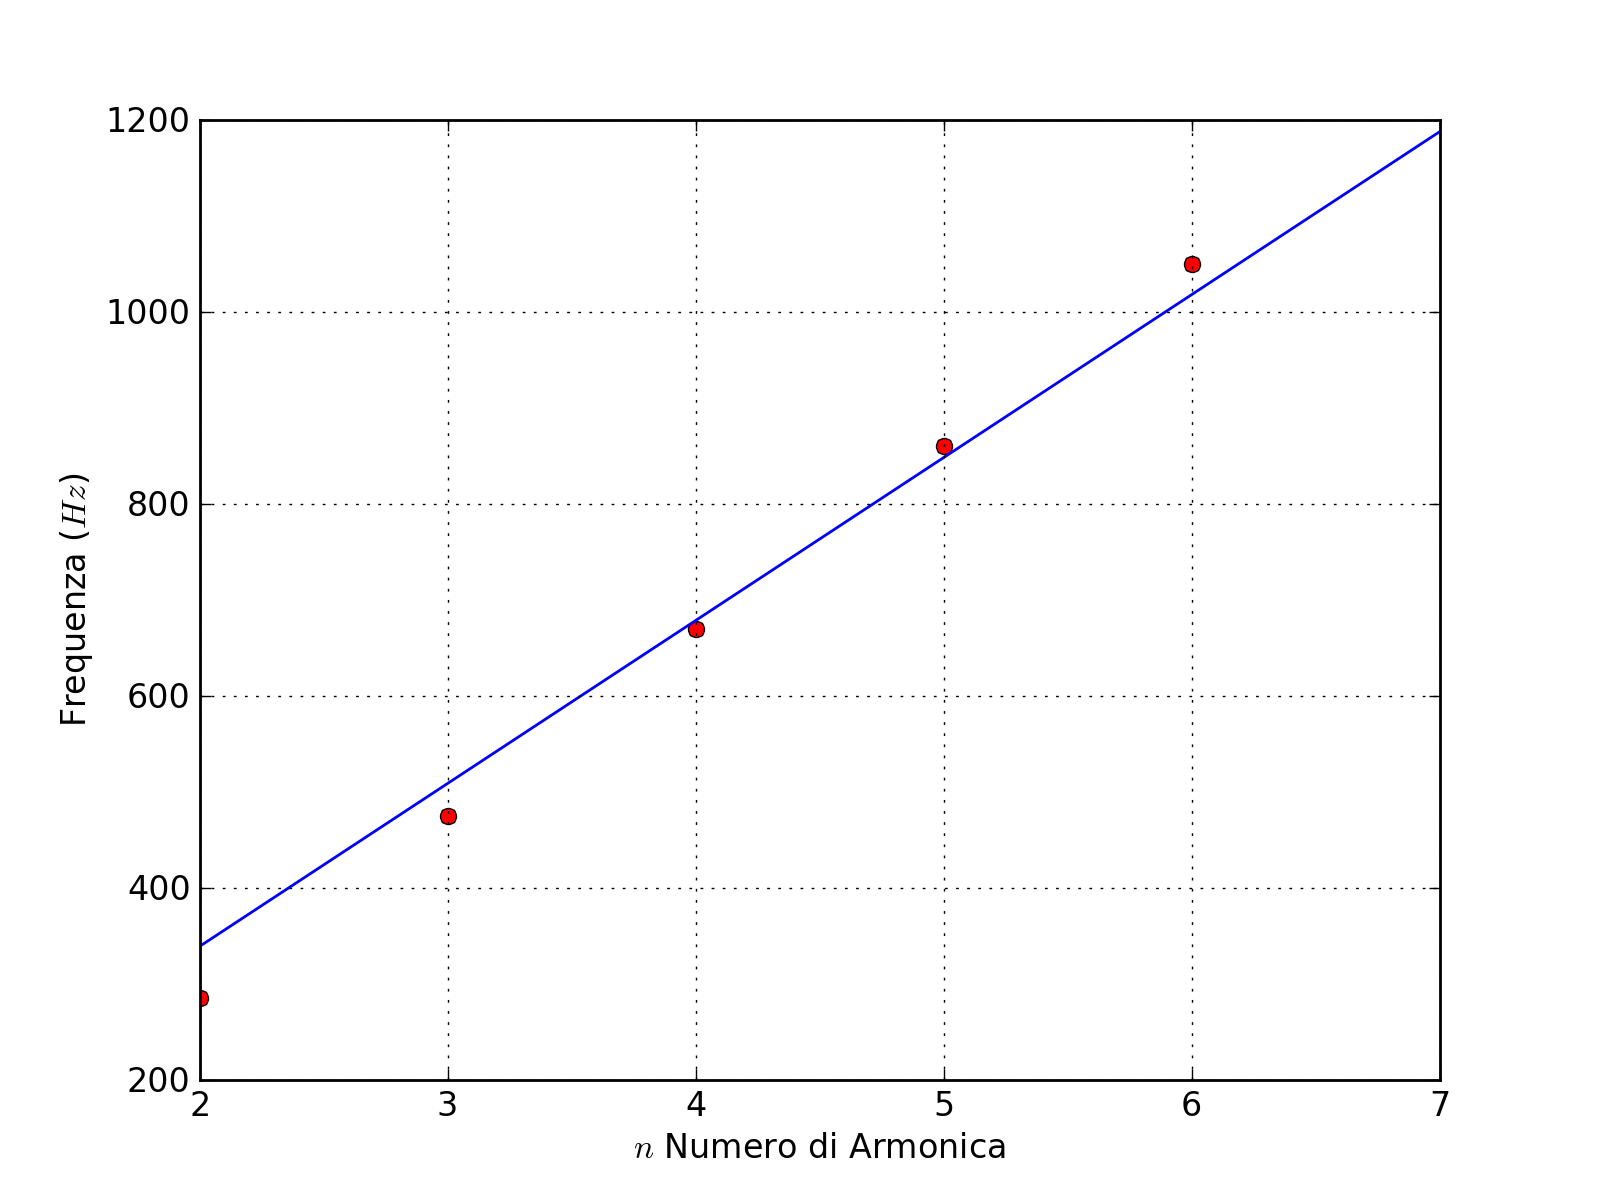
\includegraphics[scale=0.5]{../grafici/tubo/tubo2.pdf}

$m = v = 169\pm 1\ m/s$
\\

$P(\tilde{\chi}^2\geq\tilde{\chi_0}^2)=8\%$
\end{center}

\begin{center}
$\nu_0$= 475 Hz\\
\begin{tabular}{r r}
\textit{nodo 1}: & 0 cm\\
\textit{ventre 2}: & 17 cm\\
\textit{nodo 3}: & 34 cm\\
\textit{ventre 4}: & 53 cm\\
\textit{nodo 5}: & 70 cm\\
\end{tabular}
\end{center}

\subsection{Onda quadra}
La velocità del suono all'interno di un gas può essere misurata anche con un secondo metodo. Utilizzando un impulso a onda quadra e divendo la distanza totale percorsa per il tempo tra i due impulsi, otteniamo la velocità.  Per migliorare la precisione della nostra misura, abbiamo portato la risoluzione dello schermo dell'oscilloscipio ad 1 $\mu s$, in modo da poter discernere con più chiarezza la distanza tra i picchi nel grafico tempo-spazio.
Il $\Delta t$ misurato è di $4.98 \cdot 10^{-6} \ s$ e la lunghezza totale percorsa dall'impulso è $174 cm$ (2 volte la lunghezza del tubo meno la lunghezza del microfono e dello stantuffo). Ottieniamo quindi una velocità di :
$$v = 349 \pm 4 \ m/s$$
\\
con $$\sigma_v=\sqrt{\left(\frac{\sigma_t}{t}\right)+\left(\frac{\sigma_l}{L} \right)^2} \cdot v$$

\subsection{Tubo a lunghezza variabile}
Abbiamo infine verificato la dipendenza delle frequenze di risonanza dalla lunghezza del tubo.

\begin{center}
\begin{tabular}{*{5}{c|}c}
L (cm) & 60 & 65 & 70 & 75 & 80 \\
\midrule
$\nu$ (Hz) &415 & 380 & 365 & 340 & 315\\
\end{tabular}
\end{center}
Interpoliamo i dati con l'equazione:
\begin{equation}\label{tubochiuso}
\nu=\frac{(2n-1)}{L}v
\end{equation} 
usando il metodo dei minimi quadrati. Nel nostro caso la \ref{tubochiuso}, avendo $n=1$, si presenta nella forma più semmplice:
$$\nu=\frac{v}{L}$$
Poniamo $x_i=1/L_i$, $y_i=\nu_i$ ed $m=v$.

\begin{center}
%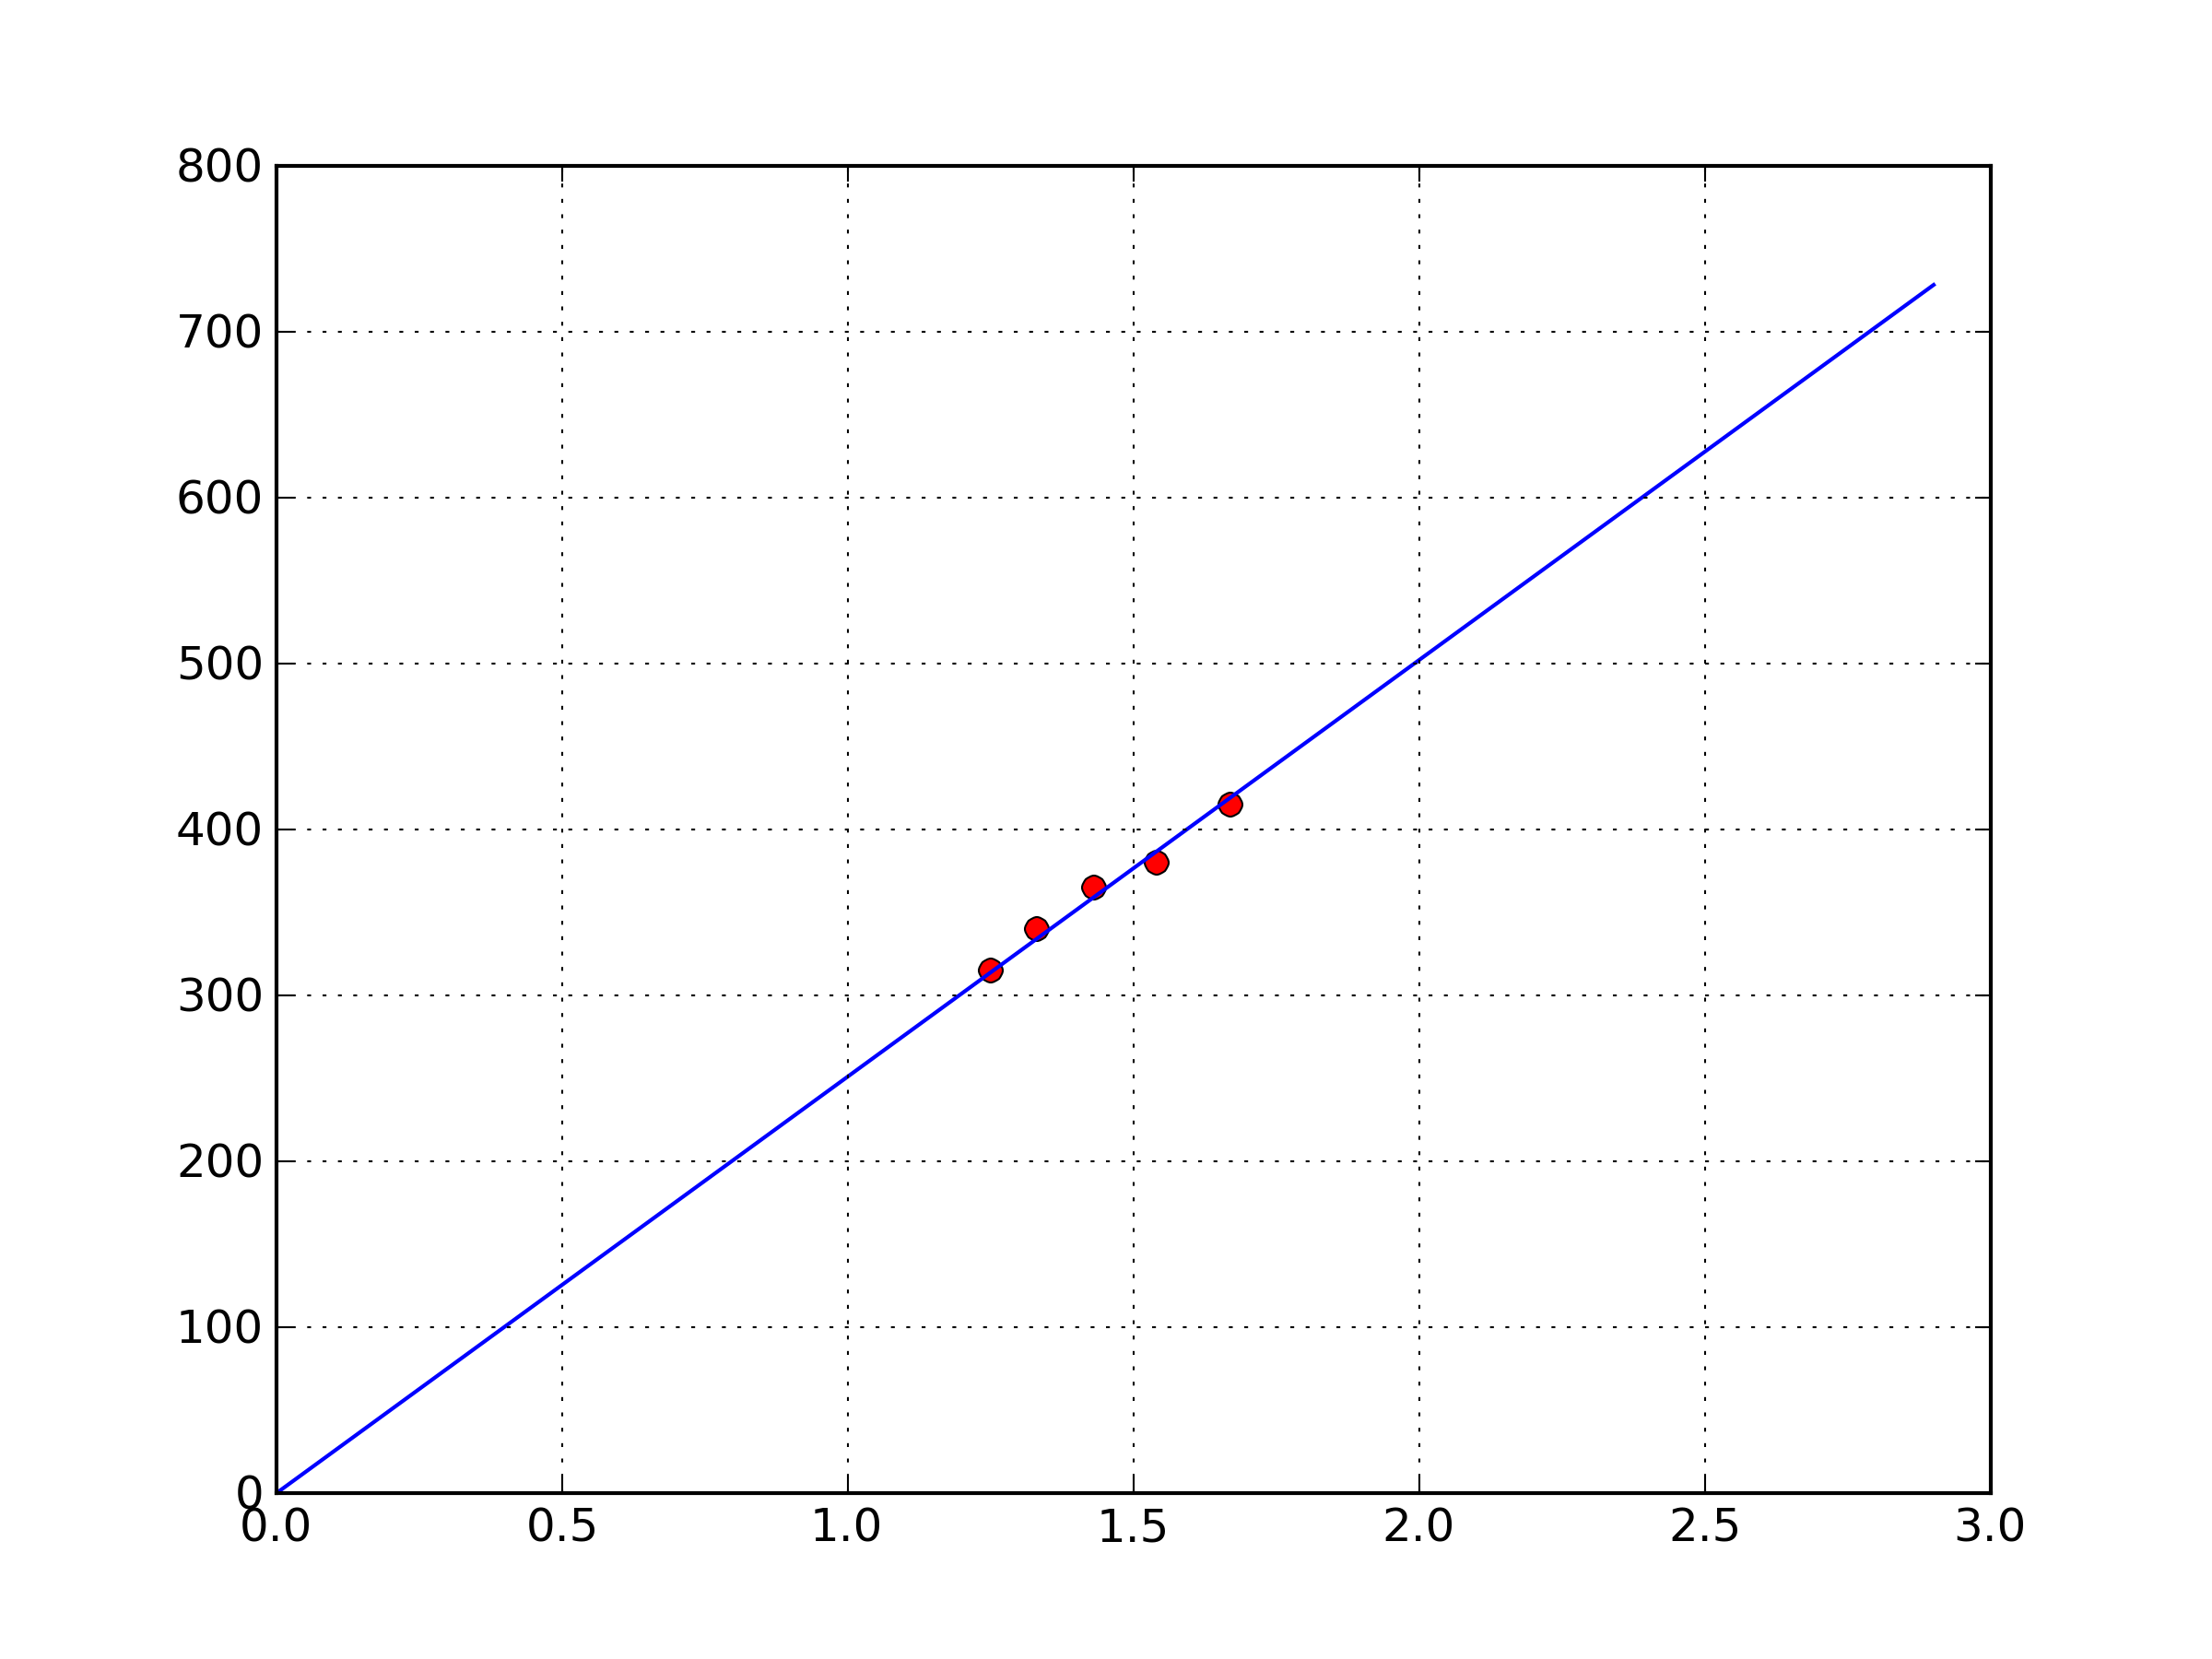
\includegraphics[scale=0.5]{../grafici/tubo/tubo3.pdf}

$m = v = 251\pm 1\ m/s$
\end{center}

\section{Tubo chiuso da ambo i lati, contenente Kripton}

$L_{tubo}$ = 147 cm\\
$D_{tubo}$ = sacchi cm
$\nu$ = 75.7 Hz
 


\begin{center}
\begin{tabular}{c|c|c|c|c|c}
$\nu$ (Hz) & 102 & 204 & 312 & 415 & 518 \\
\midrule
$n$ & 1 & 2 & 3 & 4 & 5\\
\end{tabular}
\end{center}

Interpolando i dati tramite la funzione lineare 7.1 (con correzione) otteniamo:

$$ m_2 = 104 \pm 0.5  $$ 
\\
Da questa $m$, tramite il procedimento illustrato in precedenza, calcoliamo: 
$$v = 308.4\pm0.5 m/s $$
\\
La seguente relazione:
$$v=\sqrt{\frac{\gamma RT}{M}}$$
\\
con $\gamma = \frac{C_p}{C_v}$, $R$ è la costante dei gas, $M$ la massa molare e $T$ la temperatura in gradi Kelvin, ci fornisce il valore teorico della velocità di propagazione di un'onda sonora in relazione alle caratteristiche del mezzo. 
Il risultato atteso è dunque $v=222.7 m/s$. Confrontando questo risultato con il valore misurato sperimentalmente siamo giunti alla conclusione che all'interno del tubo non era presente solo Kripton ma anche una certa percentuale di aria.

\subsection{Onda quadra}
$t_1 = 4.96 ms $\\
$t_2 = 14.6 ms $\\
$\Delta t = 9.64 ms $ \\
Applicando la formula  con $L_{tubo} = 147 cm$, otteniamo:
$$ v = 305.0 \pm \sigma m/s $$ 


